%%%%%%%%%%%%%%%%%%%%%%%%%%%%%%%%%%%%%%%%%%%%%%%%%%%%%%%%%%%%%%%%%
%
%   Template para monografia de TCC-2018 - versao 1.0.alfa
%
%%%%%%%%%%%%%%%%%%%%%%%%%%%%%%%%%%%%%%%%%%%%%%%%%%%%%%%%%%%%%%%%%
%%
%% Este template utiliza o modelo mantido pela abnt e foi baseado 
%% no abtex2-modelo-trabalho-academico.tex, v-1.9.6 laurocesar
%% Copyright 2012-2016 by abnTeX2 group at http://www.abntex.net.br/ 
%%
% -------------------------------------------------------------------
%% This work may be distributed and/or modified under the conditions 
%% of the LaTeX Project Public License, either version 1.3 of this 
%% license or (at your option) any later version. The latest version 
%% of this license is in http://www.latex-project.org/lppl.txt
%% and version 1.3 or later is part of all distributions of LaTeX
%% version 2005/12/01 or later.
%%
%% This work has the LPPL maintenance status `maintained'.
%% 
%% The Current Maintainer of this work is the abnTeX2 team, led
%% by Lauro César Araujo. Further information are available on 
%% http://www.abntex.net.br/
%%
%% This work consists of the files abntex2-modelo-trabalho-academico.tex,
%% abntex2-modelo-include-comandos and abntex2-modelo-references.bib
% -------------------------------------------------------------------
%%
%% Modelo de Monografia em conformidade com ABNT NBR 14724:2011
%%
%%%%%%%%%%%%%%%%%%%%%%%%%%%%%%%%%%%%%%%%%%%%%%%%%%%%%%%%%%%%%%%%%
%%
%% ATENÇAO para as opções:
%%
%% para modo rascunho, sem páginas brancas, use: 
%% openany, oneside, nopartblankpage
%%
%% para modo normal, com tudo que ABNT exige, use:  
%% openright, twoside, partpageblank
%%

\documentclass[
	% -- opções da classe memoir --
	12pt,			% tamanho da fonte
	openany,		% capítulos começam em qq página (isso elimina várias pág brancas)
	%openright,		% capítulos começam em pág ímpar (insere página vazia caso preciso)
	oneside,		% considera impressão de um só lado (gera menos pág brancas)
	%twoside,		% para impressão em recto e verso. Oposto a oneside
	a4paper,		% tamanho do papel. 
	% -- opções da classe abntex2 --
	%chapter=TITLE,		% títulos de capítulos convertidos em letras maiúsculas
	%section=TITLE,		% títulos de seções convertidos em letras maiúsculas
	%subsection=TITLE,	% títulos de subseções convertidos em letras maiúsculas
	%subsubsection=TITLE,% títulos de subsubseções convertidos em letras maiúsculas
	% -- opções do pacote babel --
	english,		% idioma adicional para hifenização
	%french,		% idioma adicional para hifenização
	%spanish,		% idioma adicional para hifenização
	%portuges		% o último idioma é o principal do documento
	brazil			% o último idioma é o principal do documento
	]{abntex2}


% ------------------------------------------------------------------------
%   Componente do template para monografia de TCC-2018 - versao 1.0.alfa
% ------------------------------------------------------------------------

%------------ Pacotes básicos 
\usepackage{lmodern}			% Usa a fonte Latin Modern			
\usepackage[T1]{fontenc}		% Selecao de codigos de fonte.
\usepackage[utf8]{inputenc}		% Codificacao do documento (conversão automática dos acentos)
\usepackage{lastpage}			% Usado pela Ficha catalográfica
\usepackage{indentfirst}		% Indenta o primeiro parágrafo de cada seção.
\usepackage{color}			% Controle das cores
\usepackage{graphicx}			% Inclusão de gráficos
\usepackage{microtype} 			% para melhorias de justificação
		
%------------ Pacotes adicionais
\usepackage{blindtext}			% para geração de dummy text

%------------ Pacotes de citações
\usepackage[brazilian,hyperpageref]{backref}	% Paginas com as citações na bibl
\usepackage[alf]{abntex2cite}		% Citações padrão ABNT
\usepackage{pdfpages}			% Saida em pdf

%------------ Comandos úteis
\newcommand{\aspas}[1]{``#1''}

% ----------- CONFIGURAÇÕES DE PACOTES

% Configurações do pacote backref
% Usado sem a opção hyperpageref de backref
\renewcommand{\backrefpagesname}{Citado na(s) página(s):~}
% Texto padrão antes do número das páginas
\renewcommand{\backref}{}
% Define os textos da citação
\renewcommand*{\backrefalt}[4]{
	\ifcase #1 %
		Nenhuma citação no texto.%
	\or
		Citado na página #2.%
	\else
		Citado #1 vezes nas páginas #2.%
	\fi}%
% ---

% Espaçamentos entre linhas e parágrafos 
% O tamanho do parágrafo é dado por:
\setlength{\parindent}{1.3cm}
% Controle do espaçamento entre um parágrafo e outro:
\setlength{\parskip}{0.2cm}  % tente também \onelineskip

% compila o indice
\makeindex

% ----------------------------------------------------
% Configurações de aparência do PDF final
% ----------------------------------------------------

% alterando o aspecto da cor azul
\definecolor{blue}{RGB}{41,5,195}

% informações do PDF
\makeatletter
\hypersetup{
     	%pagebackref=true,
		pdftitle={\@title}, 
		pdfauthor={\@author},
    	pdfsubject={\imprimirpreambulo},
	    pdfcreator={LaTeX with abnTeX2},
		pdfkeywords={abnt}{latex}{abntex}{abntex2}{trabalho acadêmico}, 
		colorlinks=true,       		% false: boxed links; true: colored links
    	linkcolor=blue,          	% color of internal links
    	citecolor=blue,        		% color of links to bibliography
    	filecolor=magenta,      		% color of file links
		urlcolor=blue,
		bookmarksdepth=4
}
\makeatother

% ----------------------------------------------------
% Comandos para geração de itens textuais 
% ----------------------------------------------------

\newcommand{\imprimirfichacatalografica}{

\begin{fichacatalografica}
	\sffamily
	\vspace*{\fill}					% Posição vertical
	\begin{center}					% Minipage Centralizado
	\fbox{\begin{minipage}[c][8cm]{13.5cm}		% Largura
	\small
	
	\hspace{1cm} \imprimirautor\\

	\begingroup
        \leftskip4em
        \rightskip\leftskip
	
	\imprimirtitulo  / \imprimirautor. -- \imprimirlocal, \imprimirdata.
	
	\pageref{LastPage} p. : il. (algumas color.) ; 30 cm.\\
	
	\imprimirorientadorRotulo~\imprimirorientador\\
	
	%\imprimirtipotrabalho~--~\imprimirinstituicao, \imprimirdata.\\
	Monografia para trabalho de conclusão de curso (graduação)~--~Instituto Federal 
	de Educação, Ciência e Tecnologia de Minas Gerais, Ciência da Computação, 
	Formiga, \imprimirdata.\\
	
	1. Palavra-chave1.
	2. Palavra-chave2.
	3. Palavra-chave3.
	I. \imprimirorientador.
	II. Instituto Federal de Educação, Ciência e Tecnologia de Minas Gerais.
	III. Ciência da Computação.
	IV. \imprimirtitulo 			
        \par
        \endgroup
	\end{minipage}}
	\end{center}
\end{fichacatalografica}

}

\newcommand{\imprimirerrata}{

\begin{errata}
Exemplo de errata\\[1cm]

FERRIGNO, C. R. A. \textbf{Tratamento de neoplasias ósseas apendiculares com
reimplantação de enxerto ósseo autólogo autoclavado associado ao plasma
rico em plaquetas}: estudo crítico na cirurgia de preservação de membro em
cães. 2011. 128 f. Tese (Livre-Docência) - Faculdade de Medicina Veterinária e
Zootecnia, Universidade de São Paulo, São Paulo, 2011.

\begin{table}[htb]
\center
\footnotesize
\begin{tabular}{|p{1.4cm}|p{1cm}|p{3cm}|p{3cm}|}
  \hline
   \textbf{Folha} & \textbf{Linha}  & \textbf{Onde se lê}  & \textbf{Leia-se}  \\
    \hline
    1 & 10 & auto-conclavo & autoconclavo\\
   \hline
\end{tabular}
\end{table}

\end{errata}

}

\newcommand{\imprimirfolhadeaprovacao}[1]{

\begin{folhadeaprovacao}
  \begin{center}
   {\ABNTEXchapterfont\large\imprimirautor}

   \vspace*{\fill}\vspace*{\fill}
   \begin{center}
     \ABNTEXchapterfont\bfseries\Large\imprimirtitulo
   \end{center}
   \vspace*{\fill}
    
   \hspace{.45\textwidth}
   \begin{minipage}{.5\textwidth}
       \imprimirpreambulo
   \end{minipage}%
   \vspace*{\fill}        
   \end{center}
   
   Trabalho aprovado em {#1}.
   
   \vspace{1cm}
   \hspace{4cm} BANCA EXAMINADORA    

   \assinatura{\textbf{\imprimirorientador} \\ Orientador} 
   \assinatura{\textbf{Fulano} \\ Convidado 1}
   \assinatura{\textbf{Sicrano} \\ Convidado 2}
   %\assinatura{\textbf{Professor} } %\\ Convidado 3}
   %\assinatura{\textbf{Professor} } %\\ Convidado 4}
      
   \begin{center}
    \vspace*{0.5cm}
    {\large\imprimirlocal}
    \par
    {\large\imprimirdata}
    \vspace*{1cm}
  \end{center}
  
\end{folhadeaprovacao}

}

	

\graphicspath{{./figuras/}}   	% pasta contendo todas as figuras

\nopartblankpage  		% elimina páginas em branco
% \partpageblank		% permite páginas em branco

% ----------------------------------------------------
% Informações de dados para CAPA e FOLHA DE ROSTO
% ----------------------------------------------------

\titulo{Título do TCC}
\autor{Autor do Projeto}
\local{Formiga - MG}
\data{2018}
\orientador{Nome do Orientador}
%\coorientador{se tiver}
\instituicao{%
  Instituto Federal de Educação, Ciência e Tecnologia de Minas Gerais \par
  Campus Formiga \par
  Ciência da Computação
  }
\tipotrabalho{Monografia}
% O preambulo deve conter o tipo do trabalho, o objetivo, o nome da instituição e a área de concentração 
\preambulo{Monografia do trabalho de conclusão de curso apresentado ao Instituto 
    Federal Minas Gerais - Campus Formiga, como requisito parcial para a obtenção 
    do título de Bacharel em Ciência da Computação.}

% ----------------------------------------------------
% INÍCIO DO DOCUMENTO
% ----------------------------------------------------

\begin{document}

%\selectlanguage{portuges}
\selectlanguage{brazil}

\frenchspacing  % retira espaço extra obsoleto entre as frases.

%-----------------------------------------------------
% ELEMENTOS PRÉ-TEXTUAIS
%-----------------------------------------------------
% \pretextual

\imprimircapa

\imprimirfolhaderosto*  % o comando com * indica que haverá ficha bibliográfica

%------------- Ficha catalográfica
% São os ``Dados internacionais de catalogação-na-publicação''.
% Escolha uma das opções: usar página pdf pronta (gerada pela biblioteca?!)
% ou gerar a página com o comando \imprimirfichacatalografica. 
% (Mais detalhes no preludio e documentacao do pacote abntex2.)
%
% \begin{fichacatalografica}
%     \includepdf{ficha_catalografica.pdf}
% \end{fichacatalografica}
\imprimirfichacatalografica

%------------ Errata (se houver)
% Modifique o comando \imprimirerrata no preludio e use esse comando
%\imprimirerrata

%------------ Folha de aprovação
% É um elemento obrigatório da NBR 14724/2011 (seção 4.2.1.3). 
% Você pode utilizar a página modelo até a aprovação do trabalho. 
% Após isso, gere uma página com a imagem da folha assinada pela banca,
% comente o comando \imprimirfolhadeaprovacao e use o \includepdf 
\imprimirfolhadeaprovacao{06 de junho de 2018}
% \includepdf{folhadeaprovacao_final.pdf}

%------------ Dedicatória
\begin{dedicatoria}
   \vspace*{\fill} \centering \noindent 
   \textit{ Este trabalho é dedicado ao meu pai, minha mãe,\\
   meu cachorro, meu gato, meu periquito e todo mundo.} 
   \vspace*{\fill}
\end{dedicatoria}

%------------ Agradecimentos
\begin{agradecimentos}
  Primeiramente gostaria de agradecer meus pais por tudo que fizeram,
  aos meus professores pela paciência que tiveram,
  aos cachorros pelos latidos que não deram
  e aos vigilantes pela segurança que fizeram.
\end{agradecimentos}

%------------ Epígrafe
\begin{epigrafe}
   \vspace*{\fill}
   \begin{flushright}
	\textit{\aspas{Nunca atribua à malícia/maldade o que pode ser adequadamente explicado pela estupidez.}
	(Navalha de Hanlon) }
   \end{flushright}
\end{epigrafe}

%------------ RESUMOS
\setlength{\absparsep}{18pt} % ajusta o espaçamento dos parágrafos do resumo

% resumo em português
\begin{resumo}
 A escrita da monografia é um problema clássico no Trabalho de Conclusão de Curso (TCC).
 Aqui é o lugar onde o autor explica brevemente o conteúdo do seu trabalho. Para usar este
 template é necessário instalar alguns pacotes do LaTeX, particularmente o abntex2. O pacote
 blindtex não é realmente necessário, serve apenas para gerar lero-lero neste exemplo.
 
 \textbf{Palavras-chave}: Monografia, LaTeX, TCC.
\end{resumo}

% resumo em inglês
\begin{resumo}[Abstract]
 \begin{otherlanguage*}{english}
  The writing of the monograph is a classic problem in the Course Conclusion Work.
  Here is where the author briefly explains the content of his work.
 
 \textbf{Keywords}: Monograph, LaTeX.
 \end{otherlanguage*}
\end{resumo}

% Consulte o manual da classe abntex2 para maiores 
% orientações sobre os seguintes tópicos:

%------------ Lista de ilustrações
\pdfbookmark[0]{\listfigurename}{lof}
\listoffigures*
\cleardoublepage

%------------ Lista de tabelas

%------------ Lista de abreviaturas e siglas

%------------ Lista de símbolos

%------------ Sumario
\pdfbookmark[0]{\contentsname}{toc}
\tableofcontents*
\cleardoublepage

% ----------------------------------------------------------
% ELEMENTOS TEXTUAIS
% ----------------------------------------------------------
\textual

% ----------------------------------------------------------
\chapter{Introdução}
% ----------------------------------------------------------
 
\blindtext 

\section{Justificativa}
\blindtext Exemplo de citação \cite{SCHAERF1995}.

\blindtext Mais exemplo de citação \cite{GLOVER1997}.
\blindtext Mais exemplos de citação:\cite{CESCHIA2011}, \cite{ELLOUMI2008}.

\blindtext Exemplo de citação \cite{SOUZA2004}.	

\section{Objetivos}
\subsection{Objetivo Geral}	
\blindtext
\subsection{Objetivos Específicos}	
\blinditemize[3]


% ----------------------------------------------------------
\chapter{Fundamentação Teórica}
% ----------------------------------------------------------

\blindtext 

\section[Conceito1]{Primeiro Conceito}

\blindtext

\blindtext[2]

\blindtext

A figura~\ref{fig-tostines} ilustra primeiro material conhecido causador do Efeito Tostines.

\begin{figure}[!htb]
	\centering
	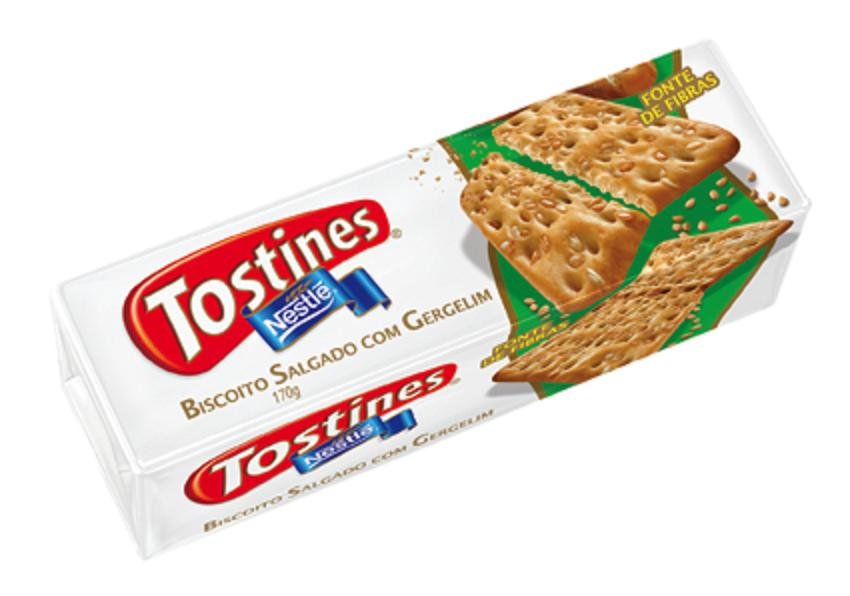
\includegraphics[scale=0.45]{tostines.jpg}
	\caption{Exemplo de objeto causador de Efeito Tostines}
	\label{fig-tostines}
\end{figure}

\blindtext[2]

\section[Conceito2]{Segundo Conceito}

\blindtext

\blindtext[2]

\blindtext
		


% ----------------------------------------------------------
\chapter{Desenvolvimento}
% ----------------------------------------------------------

\blindtext 

\section[Parte1]{Primeira Parte}

\blindtext

\blindtext[2]

\blindtext[3]

\section[Parte2]{Segunda Parte}

\blindtext

\blindtext[2]

\blindtext


% ----------------------------------------------------------
\chapter{Conclusão}
% ----------------------------------------------------------

\blindtext

\blindtext[2]


% ----------------------------------------------------------
\chapter{Trabalhos futuros}
% ----------------------------------------------------------

\blindtext

\blindenumerate[4]

\blindtext


\phantompart

% ----------------------------------------------------------
% ELEMENTOS PÓS-TEXTUAIS
% ----------------------------------------------------------
\postextual

% Referências bibliográficas
\bibliography{monografia}

% Consulte o manual da classe abntex2 para orientações 
% sobre os seguintes tópicos opcionais:

%------------ Glossário

%------------ Apêndices

%------------ Anexos

% INDICE REMISSIVO
\phantompart
\printindex

\end{document}
\grid
